%  LaTeX support: latex@mdpi.com 
%  For support, please attach all files needed for compiling as well as the log file, and specify your operating system, LaTeX version, and LaTeX editor.

%=================================================================
\documentclass[journal,article,submit,moreauthors,pdftex]{Definitions/mdpi} 

% For posting an early version of this manuscript as a preprint, you may use "preprints" as the journal and change "submit" to "accept". The document class line would be, e.g., \documentclass[preprints,article,accept,moreauthors,pdftex]{mdpi}. This is especially recommended for submission to arXiv, where line numbers should be removed before posting. For preprints.org, the editorial staff will make this change immediately prior to posting.

%--------------------
% Class Options:
%--------------------
%----------
% journal
%----------
% Choose between the following MDPI journals:
% acoustics, actuators, addictions, admsci, adolescents, aerospace, agriculture, agriengineering, agronomy, ai, algorithms, allergies, analytica, animals, antibiotics, antibodies, antioxidants, appliedchem, applmech, applmicrobiol, applnano, applsci, arts, asi, atmosphere, atoms, audiolres, automation, axioms, batteries, bdcc, behavsci, beverages, biochem, bioengineering, biologics, biology, biomechanics, biomedicines, biomedinformatics, biomimetics, biomolecules, biophysica, biosensors, biotech, birds, bloods, brainsci, buildings, businesses, cancers, carbon, cardiogenetics, catalysts, cells, ceramics, challenges, chemengineering, chemistry, chemosensors, chemproc, children, civileng, cleantechnol, climate, clinpract, clockssleep, cmd, coatings, colloids, compounds, computation, computers, condensedmatter, conservation, constrmater, cosmetics, crops, cryptography, crystals, curroncol, cyber, dairy, data, dentistry, dermato, dermatopathology, designs, diabetology, diagnostics, digital, disabilities, diseases, diversity, dna, drones, dynamics, earth, ebj, ecologies, econometrics, economies, education, ejihpe, electricity, electrochem, electronicmat, electronics, encyclopedia, endocrines, energies, eng, engproc, entropy, environments, environsciproc, epidemiologia, epigenomes, fermentation, fibers, fire, fishes, fluids, foods, forecasting, forensicsci, forests, fractalfract, fuels, futureinternet, futuretransp, futurepharmacol, futurephys, galaxies, games, gases, gastroent, gastrointestdisord, gels, genealogy, genes, geographies, geohazards, geomatics, geosciences, geotechnics, geriatrics, hazardousmatters, healthcare, hearts, hemato, heritage, highthroughput, histories, horticulturae, humanities, hydrogen, hydrology, hygiene, idr, ijerph, ijfs, ijgi, ijms, ijns, ijtm, ijtpp, immuno, informatics, information, infrastructures, inorganics, insects, instruments, inventions, iot, j, jcdd, jcm, jcp, jcs, jdb, jfb, jfmk, jimaging, jintelligence, jlpea, jmmp, jmp, jmse, jne, jnt, jof, joitmc, jor, journalmedia, jox, jpm, jrfm, jsan, jtaer, jzbg, kidney, land, languages, laws, life, liquids, literature, livers, logistics, lubricants, machines, macromol, magnetism, magnetochemistry, make, marinedrugs, materials, materproc, mathematics, mca, measurements, medicina, medicines, medsci, membranes, metabolites, metals, metrology, micro, microarrays, microbiolres, micromachines, microorganisms, minerals, mining, modelling, molbank, molecules, mps, mti, nanoenergyadv, nanomanufacturing, nanomaterials, ncrna, network, neuroglia, neurolint, neurosci, nitrogen, notspecified, nri, nursrep, nutrients, obesities, oceans, ohbm, onco, oncopathology, optics, oral, organics, osteology, oxygen, parasites, parasitologia, particles, pathogens, pathophysiology, pediatrrep, pharmaceuticals, pharmaceutics, pharmacy, philosophies, photochem, photonics, physchem, physics, physiolsci, plants, plasma, pollutants, polymers, polysaccharides, proceedings, processes, prosthesis, proteomes, psych, psychiatryint, publications, quantumrep, quaternary, qubs, radiation, reactions, recycling, regeneration, religions, remotesensing, reports, reprodmed, resources, risks, robotics, safety, sci, scipharm, sensors, separations, sexes, signals, sinusitis, smartcities, sna, societies, socsci, soilsystems, solids, sports, standards, stats, stresses, surfaces, surgeries, suschem, sustainability, symmetry, systems, taxonomy, technologies, telecom, textiles, thermo, tourismhosp, toxics, toxins, transplantology, traumas, tropicalmed, universe, urbansci, uro, vaccines, vehicles, vetsci, vibration, viruses, vision, water, wevj, women, world 

%---------
% article
%---------
% The default type of manuscript is "article", but can be replaced by: 
% abstract, addendum, article, book, bookreview, briefreport, casereport, comment, commentary, communication, conferenceproceedings, correction, conferencereport, entry, expressionofconcern, extendedabstract, datadescriptor, editorial, essay, erratum, hypothesis, interestingimage, obituary, opinion, projectreport, reply, retraction, review, perspective, protocol, shortnote, studyprotocol, systematicreview, supfile, technicalnote, viewpoint, guidelines, registeredreport, tutorial
% supfile = supplementary materials

%----------
% submit
%----------
% The class option "submit" will be changed to "accept" by the Editorial Office when the paper is accepted. This will only make changes to the frontpage (e.g., the logo of the journal will get visible), the headings, and the copyright information. Also, line numbering will be removed. Journal info and pagination for accepted papers will also be assigned by the Editorial Office.

%------------------
% moreauthors
%------------------
% If there is only one author the class option oneauthor should be used. Otherwise use the class option moreauthors.

%---------
% pdftex
%---------
% The option pdftex is for use with pdfLaTeX. If eps figures are used, remove the option pdftex and use LaTeX and dvi2pdf.

%=================================================================
% MDPI internal commands
\firstpage{1} 
\makeatletter 
\setcounter{page}{\@firstpage} 
\makeatother
\pubvolume{1}
\issuenum{1}
\articlenumber{0}
\pubyear{2021}
\copyrightyear{2020}
%\externaleditor{Academic Editor: Firstname Lastname} % For journal Automation, please change Academic Editor to "Communicated by"
\datereceived{} 
\dateaccepted{} 
\datepublished{} 
\hreflink{https://doi.org/} % If needed use \linebreak
%------------------------------------------------------------------
% The following line should be uncommented if the LaTeX file is uploaded to arXiv.org
%\pdfoutput=1

%=================================================================
% Add packages and commands here. The following packages are loaded in our class file: fontenc, inputenc, calc, indentfirst, fancyhdr, graphicx, epstopdf, lastpage, ifthen, lineno, float, amsmath, setspace, enumitem, mathpazo, booktabs, titlesec, etoolbox, tabto, xcolor, soul, multirow, microtype, tikz, totcount, changepage, paracol, attrib, upgreek, cleveref, amsthm, hyphenat, natbib, hyperref, footmisc, url, geometry, newfloat, caption

%=================================================================
%% Please use the following mathematics environments: Theorem, Lemma, Corollary, Proposition, Characterization, Property, Problem, Example, ExamplesandDefinitions, Hypothesis, Remark, Definition, Notation, Assumption
%% For proofs, please use the proof environment (the amsthm package is loaded by the MDPI class).

%=================================================================
% Full title of the paper (Capitalized)
\Title{The Effects of Adversarial Training on the Safety of Classifictaion Models}

% MDPI internal command: Title for citation in the left column
\TitleCitation{Title}

% Author Orchid ID: enter ID or remove command
\newcommand{\orcidauthorA}{0000-0000-0000-000X} % Add \orcidA{} behind the author's name
%\newcommand{\orcidauthorB}{0000-0000-0000-000X} % Add \orcidB{} behind the author's name

% Authors, for the paper (add full first names)
\Author{Handong Kim $^{1,\dagger}$\orcidA{} and Jongdae Han $^{2,}$*}

% MDPI internal command: Authors, for metadata in PDF
\AuthorNames{Handong Kim and Jongdae Han}

% MDPI internal command: Authors, for citation in the left column
\AuthorCitation{Lastname, F.; Lastname, F.; Lastname, F.}
% If this is a Chicago style journal: Lastname, Firstname, Firstname Lastname, and Firstname Lastname.

% Affiliations / Addresses (Add [1] after \address if there is only one affiliation.)
\address{%
$^{1}$ \quad Affiliation 1; sw.engineering@kakao.com\\
$^{2}$ \quad Affiliation 2; elvenwhite@smu.ac.kr}

% Contact information of the corresponding author
\corres{Correspondence: elvenwhite@smu.ac.kr; Tel.: (optional; include country code; if there are multiple corresponding authors, add author initials) +xx-xxxx-xxx-xxxx (F.L.)}

% Current address and/or shared authorship
\firstnote{Current address: Affiliation 3} 
% \secondnote{These authors contributed equally to this work.}
% The commands \thirdnote{} till \eighthnote{} are available for further notes

%\simplesumm{} % Simple summary

%\conference{} % An extended version of a conference paper

% Abstract (Do not insert blank lines, i.e. \\) 
\abstract{A single paragraph of about 200 words maximum. For research articles, abstracts should give a pertinent overview of the work. We strongly encourage authors to use the following style of structured abstracts, but without headings: (1) Background: place the question addressed in a broad context and highlight the purpose of the study; (2) Methods: describe briefly the main methods or treatments applied; (3) Results: summarize the article's main findings; (4) Conclusion: indicate the main conclusions or interpretations. The abstract should be an objective representation of the article, it must not contain results which are not presented and substantiated in the main text and should not exaggerate the main conclusions.}
% AI가 일상 생활에서 많이 사용되는 추세이지만 중요 요소 중 하나인 비기능적 요구사항 검증에 대한 연구가 거의 이루어지지 않았다.
% 논문에서는 분류 모델에 대해 적대적 학습을 활용하여 적대적 학습이 인공지능의 비기능적 요구사항 중 하나인 안전성에 미치는 영향을 평가, 안전성을 검증하기 위한 방법으로 사용할 수 있음을 주장한다.
% 서로 다른 데이터셋 및 모델에 대해서 적대적 학습이 정확도와 안전성에 미치는 영향을 확인, 정확도(성능)가 떨어지는 것에 비해 큰 폭의 안전성 상승을 확인할 수 있었고 이를 통해 적대적 예시를 만드는 것이 안전성 검증을 위한 요소로 사용될 수 있음을 증명하였다.
% 나아가 서로 다른 적대적 예시 포함 비율 실험을 통하여 중요시하는 비기능적 요구사항에 따라 적대적 예시 포함 비율을 조정하는 것 또한 비기능적 요구사항을 검증할 수 있는 요소 중 하나로 활용될 수 있음을 증명하였다.

% Keywords
\keyword{keyword 1; keyword 2; keyword 3 (List three to ten pertinent keywords specific to the article; yet reasonably common within the subject discipline.)} 

% The fields PACS, MSC, and JEL may be left empty or commented out if not applicable
%\PACS{J0101}
%\MSC{}
%\JEL{}

%%%%%%%%%%%%%%%%%%%%%%%%%%%%%%%%%%%%%%%%%%
% Only for the journal Diversity
%\LSID{\url{http://}}

%%%%%%%%%%%%%%%%%%%%%%%%%%%%%%%%%%%%%%%%%%
% Only for the journal Applied Sciences:
%\featuredapplication{Authors are encouraged to provide a concise description of the specific application or a potential application of the work. This section is not mandatory.}
%%%%%%%%%%%%%%%%%%%%%%%%%%%%%%%%%%%%%%%%%%

%%%%%%%%%%%%%%%%%%%%%%%%%%%%%%%%%%%%%%%%%%
% Only for the journal Data:
%\dataset{DOI number or link to the deposited data set in cases where the data set is published or set to be published separately. If the data set is submitted and will be published as a supplement to this paper in the journal Data, this field will be filled by the editors of the journal. In this case, please make sure to submit the data set as a supplement when entering your manuscript into our manuscript editorial system.}

%\datasetlicense{license under which the data set is made available (CC0, CC-BY, CC-BY-SA, CC-BY-NC, etc.)}

%%%%%%%%%%%%%%%%%%%%%%%%%%%%%%%%%%%%%%%%%%
% Only for the journal Toxins
%\keycontribution{The breakthroughs or highlights of the manuscript. Authors can write one or two sentences to describe the most important part of the paper.}

%%%%%%%%%%%%%%%%%%%%%%%%%%%%%%%%%%%%%%%%%%
% Only for the journal Encyclopedia
% \encyclopediadef{Instead of the abstract}
% \entrylink{The Link to this entry published on the encyclopedia platform.}
%%%%%%%%%%%%%%%%%%%%%%%%%%%%%%%%%%%%%%%%%%
\begin{document}
\setcounter{section}

\section{Introduction}

% 기능적 요구사항 및 비기능적 요구사항에 대한 간단한 설명과 검증하는 것이 왜 중요한지에 대한 설명 추가
% 기존 소프트웨어에서 요구사항을 검증하는 방법에 대한 내용 순서 조정
% AI 요구사항 검증 및 문제 제시에 대한 내용 수정
Software requirements are one of the important factors affects software quality.
If we verify the requirements in early step of software development life cycle, the more likely to develop high quality software as well as to save resources which may be needed to resolve future problems.
Requirements can be divided into functional requirements and non-functional requirements(NFRs).
Functional requirements are requirements for whether the software properly provides the functions that users want.
NFRs are requirements excluding functional requirements. NFRs include the performance(whether software performs the desired behavior), security, safety(whether the execution result of software is safe), reliability(transparency, whether software can be trusted), and etc. % reference 정리
It can be said that it is essential to verifty not only functional requirements but also NFRs for high quality software.

% 기존 소프트웨어에서의 요구사항 검증 방법
Existing software has been quickley verifying requirements through many methods such as V model which makes detailed documentation and testing at each stage of the software development life cycle.
In existing software, it is possible for people to directly check the operation of code, so functional requirements as well as non-functional requirements(NFRs) can be verified through code.\

% 인공지능에서 비기능적 요구사항의 중요성 및 문제 제시
However, with the advent of Deep Neural Network(DNN), artificial intelligence(AI), which has different characteristics with existing software that appeared throughout society, is difficult to verify requirements by methods used in existing software.
Performance, which is one of the NFRs, can be verified to some extent through accuracy or F1-score measurement. However, other NFRs like safety are difficult to verify.
The reason why it is difficult to use the verification methods of existing software in AI is because AI operated as black box model. In existing software, these NFRs could be verified through code, but in AI, it is difficult to verify them because it counldn't identify the operation of the code.
In AI, verification of NFRs is important especially in the areas that can have a fatal impact on humans such as autonomous driving, medical diagnosis, and finance.
If NFRs such as safety, security, and transparency are not guaranteed, not only fatal human problems but also other problems such as legal problems about liability may arise.
Nevertheless, the quality assessment of AI is mainly done only on the performance corresponding to how well AI through methods such as accuracy and F1-score and NFRs are rarely dealt with.

% TODO :: Related works 정리 후 수정 예정(이 문단 전체)
% 주요 내용 : 학습 데이터 공정성을 통해 개선하려는 연구들이 진행되었음. 다른 방법(xai, adversarial training)을 통해 AI의 성능을 개선하려는 연구들이 있었는데, 이러한 연구들에서 비기능적 요구사항 검증 방법에 대한 실마리를 잡을 수 있다.
There are some studies for verifying NFRs of AI. Some of studies' goal is not mainly for verifying NFRs of AI, but there are some points thar can be said to be the purpose of study is for verifying NFRs of AI.
The Microsoft proposed Fairlearn[], an open source project to ensure fairness of machine learning models, to improve unfair situations that may occur when the fairness of training data is not guaranted.
Other studies carried out include studies on explainable AI(XAI). These studies were conducted to enable people to understand the process of deriving results of AI. In other words, it can be said that it is a process that can verify the transparency of the results derived by AI.
There are also studies of adversarial examples and adversarial training. These studies show that machine learning is inevitably vulnerable to adversarial examples due to its' learning algorithm and suggest several methods to counter adversarial attacks.
Althogh the purpose of these stuides is to maintain or imporve the performance of the model from adversarial examples, it can be interpreted as a verification method to properly classify adversarial examples that threaten the safety of learned models.
While these studies made contributions such as revealing the learning process of the model and responding well to adversarial examples, it is somewhat insufficient to say that they contributed to the verification of AI NFRs.
Therefore, in this paper, we proceed with a study to verify NFRs of AI especially safety of classification model using adversarial training, inspired by the other interpretation of previous studies we said above.
% 특히 적대적 학습을 통한 적대적 예시에 대한 robust한 결과를 얻어낼 수 있다는 점으로부터, 소프트웨어의 안전성 검증과 연관을 지을 수 있을 것이라고 생각하였다. 
% 이를 확인하기 위해 논문에서는 분류 모델과 이에 대한 자세한 내용은 3장에 대해서 다룬다.
There are the purpose of AI is very diverse and the required NFRs vary according to the purpose, this paper conducted a study on the safety of classification model. The definition of safety and detail purpose of this paper are covered in chapter 3.
In this paper, we assume that the safety of classification model can be improved by using adversarial examples as a part of datas for learning(adversarial training).
For proving this, we set up the following research questions(RQ).

\begin{description}
    \item[RQ1.]	Can classification model correctly classify adversarial examples by adversarial training?
    \item[RQ2.]	Does it show the same results as RQ1 for the dataset related to safety?
    \item[RQ3.] Does adversarial training affect safety performance regardless of model structure?
    \item[RQ4.]	At what rate will learning with adversarial examples perform best?
\end{description}

Through experiments to answer each RQ, we were able to make the following contributions in this paper.

% main 기법이 아닌 결과에 따른 선택적으로 main process로 사용할 수 있거나 성능 향상을 위한 보조적인 수단으로 활용할 수 있음을 어필₩
\begin{enumerate}
    \item	We have shown that adversarial training can lead to improved safety performance. Depending on the experimental results, it can be seen that safety is improved by 2 to 40\%.
    \item	We have shown that adversarial training can be one of the factors to be verified for the safety of AI. Experimental results show that adversarial training can affect safety improvement, which can be one of the verification methods to ensure safety by pre-generating adversarial examples and utilizing the adversrail exmaples generated.
    \item   We have shown that adversarial training can be utilized as one of the factores that can verify safety regradless of model structure. Experimental results show that there was a differences in numerical values depending on the model structure, showing the same tendency.
    \item	We propose a process to adjust the ratio of inclusion adversarial example in training datasets according to the preferential requirements. Experimental results with different adversarial example inclusion ratios demonstrated that adversarial inclusion ratios plays key roles for trade-off between accuracy and safety.
\end{enumerate} 

The contents of the paper are structured as follows. In chapter 2, we deals with the introduction of previous studies conducted for verification methods for AI NFRs.
In chapter 3, we deals with the definition of safety and experimental design that we would like to see in our paper.
In chapter 4, we introduces exmperiments conducted according to designed experimental methods.
In chapter 5, we analyze the experiental results and make a discussion of experimental results.
In chapter 6, we intoduces the conclusion of the paper and future work.

%%%%%%%%%%%%%%%%%%%%%%%%%%%%%%%%%%%%%%%%%%
\section{Related works}

There are prior studies that directly or indirectly affected the field of NFRs verification of AI.

% TODO ::
% \subsection{Importance of NFRs in AI}
% AI의 비기능적 요구사항이 중요한 이유에 대한 논문들에 대해서 기술 Concrete problems in AI safety 논문을 중심으로 찾을 예정
% the studies on the fairness of training data 항목 편입 예정
% Introduction의 관련 연구 언급 부분에 대해서도 수정할 예정

\subsection{The studies on the fairness of training data}

AI learns the features of the data and derives the results of the input data based on the learned features. Due to theses characteristics, if bias exists in the training data set, discriminatory results can be produced for each individuals or group use AI.
This can be said to be the result of not satisfying fairness, one of the AI NFRs that requires every users to achieve the same results.
[] points out that the bias in training dataset can lead to discriminatory results according to features such as race, gender, and age of each individuals.
To solve this problem, they proposed a statistical method to identify the discriminating elements of the training dataset, and furthermore, they argued that it is important to keep the fairness of AI as data bias is related to privacy.
[] proposed the problem of discrimantation that the discriminatory feature of dataset can have on the group using AI and a method to solve the problem.
To improve the fairness of the AI, [] and Microsoft's Fairlearn find and remove factors that hinder fairness, such as bias, which exists in training dataset.

\subsection{Explainable Ariticial Intelligence(XAI)}

The main purpose of the sutdies conducted on XAI is not to verify the AI NFRs.
However, through these studies, people were able to know the learning and result derivation process of AI, which is directly related to the transparency of the AI, so they were included as a related studies.
One of the characteristics of AI is that it works in a black box. People cannot check what features AI learns from training data and what process it goes through to derive results.
This raises the problem that the results derived by AI cannot be trusted unconditionally.
In particular, it is more important to solve these problems in fields where the results of AI have a large impact on humans, such as autonomous driving and medical diagnosis.
In order to solve this problems, XAI conducted research to enbalbe humans to check the process of AI learning and the process of deriving results.
Studies in [], [] define the concept of XAI and introduce the methodology used for XAI to organize previous studies that have benn conducted for XAI.

\subsection{Adversarial examples and adversarial attacks}

The main purpose of the studies conducted on adversarial examples and adversarial training is not to verify the AI NFRs.
However, in the study of [], it was noted that:
\begin{quote}
   " A good response to adversarial examples is an important part of the safety issue of AI"
\end{quote}
it can be seen that adversarial examples are related with safety of AI.
[], [] show that the characteristics of the learning algorithm of AI are bound to vulnerable to adversarial examples, which behave as adversarial examples regradless of the structure and training data of the models.
[] proposes an FGSM that uses gradients from the learning process to generate adversarial examples.
[] demonstrated through experiments that when the original data used for learning was captured using a smartphone camera and applied to the model, it can behave like an adversarial examples. It has been shown to be effective in the real environment rather than the expoerimental environmnet.
[] proposes a mehtod for adversarial attacks in a black box environment\_with no information about the network and no information about the training dataset\_, rather than the existing white-box approach\_knows the structure of network and tranining datasets\_. \\

Several studies on NFRs have benn conducted, and even for studies that do not have the main purpose of NFRs, the attributes related to the verification of NFRs can be confirmed.
Inspired by theses studies, we proceed with the research of the thesis.

%%%%%%%%%%%%%%%%%%%%%%%%%%%%%%%%%%%%%%%%%%
\section{Definition of safety and Experimental design} % Overview of experiments

% Introduction에서 생략하거나 자세히 설명하지 않은 부분에 대한 내용 추가
% 왜 안전성인가 ? 왜 분류 모델인가 ?
% 안전성의 정의와 왜 안전성을 해당 요소와 같이 정의하였는지

In this chapter, we discusses what is the safety of AI in this paper and how the we designed the experiment to answer the RQs.

\begin{figure}[H]
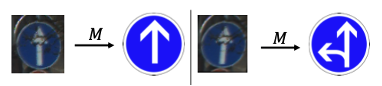
\includegraphics[width=13 cm]{Definitions/example-of-adversarial.png}
\caption{Examples of adversarial examples.\label{example-of-adversarial}}
\end{figure}   

AI needs to ensure minimum safety regradless of its purpose. In the field where AI is applied, actual input data may not exist in the dataset used for training.
In addition, AI is likely to suffer from multiple threats in real-world applications and adversarial attacks(adversarial examples) are one of the examples.
Examples of adversarial attacks can be seen in Figure~\ref{example-of-adversarial}. Both signs appear to be the same sign in human eyes. However, the right one with adversarial attack is not properly classified compared to left one in Figure is classified correctly.
Models applied to fields where the results can have a significant impact on humans, such as autonomous driving and medical diagnosis, can cause fatal safety problems if they do not properly respond to adversarial attacks. Therefore, in such a field, it is important to respond well to adversarial attacks and to ensure safety.
Through this, the paper defiend safety as bellows.

\begin{quote}
    "\textit{\textbf{Safety}} is the measure of whether the model responds appropriately to data with untrained features or to data that has been adversarial attacked to obtain incorrect results from the model."
\end{quote}

Learning all data and adversarial examples that may occur in the environment in which the model is applied is the best way to ensure safety.
However, in reality, it is difficult to collect all data on all situations, and even if it collected, it is difficult because it consumes a lot of resources to process and train the data.
Then, in a situation where it is impossible to learn all data, which data should be learned first to ensure minimum safety?
In the paper, we assumed that adversarial examples are given the highest priority and are the data that should be learned.
This is because adversarial examples are data designed for the purpose of causing problems or confusing the results of the model.
For data under other conditions, it cannot be said that the results derived from the model unconditionally cause problems.
On the other hand, adversarial examples are very likely to cause problems with the model's results.
For example, in a traffic signs for autonomous driving, there may be data to cause problems as shown in Figure~\ref{example-of-adversarial}, whereas there may be data that does not necessarily lead to problems, such as traffic signs with natural environment(sunlight, fog, etc.).
Another reason is the difficulty of creating and configuring datasets. It is difficult to generate corresponding data because there are too many conditions for the data that can occur in the environment in which the model is applied.
On the other hand, in the case of a adversarial examples, many studies on adversarial attack methods for this purpose have been conducted, so it is relatively easy to generate compared to the previous data.
For these reasons, the paper thought adversarial training is a way to ensure minimum safety of AI, and tried to prove it through experiments.
If adversarial training allows the model to better respond to adversarial examples\_improves safety performance\_, it can be used as a way to verify whether safety is guaranteed in advance by preparing adversarial examples before training and mixing them with the training data. \\

In order to show this through experiments, we first prepared different kinds of datasets and used the prepared datasets to generate adversarial datasets with different degrees of transformation \begin{math}\epsilon\end{math}.
The reason for the preparing several \begin{math}\epsilon\end{math} is to check the effect of \begin{math}\epsilon\end{math} on safety performance. If the \begin{math}\epsilon\end{math}is too small, the safety performance will not improve because there is little difference from the original data, so it cannot classify adversarial examples well. If the (\begin{math}\epsilon\end{math}) is too large, the features of the original data cannot be learned properly, resulting in poor performance such as the accuracy of the existing model.
In addition, when generating datasets for adversarial training, the size of the training dataset was kept the same as the size of the existing training dataset.
This is because increasing the number of data does not necessarily lead to improved performance of the model, as well as requiring additional resources to learn it.
Furthermore, in order to show at what ratio adversarial examples should be included for safety verification in the data preparation stage, the experiment was conductted by setting the mixing ratio of the original data and the adversarial examples differently.
At this time, if adversarial training is executed, the number of original training data was reduced, and thus the accuracy, which is one of the performance evaluation measures of the model for accurately classifying the original evalutaiton datset, may decrease.
It is important improving safety, but accuracy can be more important than safety at some moment that depends on the purpose of the model. So, it is also necessary to ensure accuracy as well as safety. 
Therefore, in order to maintain the accuracy of the model learned with original dataset with the appropriate resources, we chose the method of mixing the original data and adversarial examples at an appropriate ratio while preserving the size of the traning dataset.
To show this, the accuracy is additionaly selected as a measure of performance evaluation.
Althogh both accuracy and safety are measures of performance of how well a given data is classified, but we devided measures by the target evaluation datasets to distinguish them on a scale with different meanings.
Accuracy represents how well model classifies the {\it original} evaluation dataset, and safety represents how well model classifies the {\it adversarial} evaluation dataset, which is considered to be threatening to the model according to the definition given above.
In the belief that the results may differ depending on the characteristics of the model's structure, we also prepared learning models with different types of structures. 
Detail informations about dataset, adversarial attack method, accuracy, safety, models and experimental methods will be discussed in chapter 4.

%%%%%%%%%%%%%%%%%%%%%%%%%%%%%%%%%%%%%%%%%%
\section{Methodology}

We conducted experiments under different conditions to answer the RQs. For the experiment, we parpared datasets with three different characteristics and models with three different structures.
Section 4.1 introduces a introduction to the datasets and models used in our experiment and the reason why they were selected.
Section 4.2 introduces a breif introduction to FGSM for generating adversarial examples and the reason why is was selected.
Section 4.3 introduces each process of the experiment designed in chapter 3.

\subsection{Datasets and Models}

\subsection{Datasets}

% 각 데이터 셋을 사용한 이유에 대해서 작성
For the experiments, three dataset were used: CIFAR-10, CIFAR-100, and GTSRB. The CIFAR-10 dataset consists of a total 60,000 datas in 10 classes, each contains 6,000 datas with 3 channels and \begin{math}{32\times 32}\end{math} size.
Of these, 5,000 datas are used for training and last datas used for evaluation.

\begin{figure}[H] 

\includegraphics[width=5 cm]{Definitions/logo-mdpi}
\caption{Some datas from each dataset.\label{fig3}}
\end{figure} 

% 그림에서 확인할 수 있다는 내용 추가
You can see the examples of used datasets in Figure~\ref{fig3}.
The CIFAR-100 dataset consists of a total 60,000 datas in 100 classes, each contains 600 datas with 3 channels and \begin{math}{32\times 32}\end{math} size. Of these, 500 datas are used for training and last datas used for evaluation.
The CIFAR-10 and CIFAR-100 datasets were used for experiment to answer RQ1, which corresponds to the most basic hypothesis established in our paper.
This is due to the difference between CIFAR-10 and CIFAR-100. The CIFAR-10 has a large number of data for a small classes, which is likely for the model to learn features for each class. On the other hand, CIFAR-100 has a small number of data for many classes, so model is less likely to learn features for each class.
If it is possible to identify the improvement of safety through adversarial training for datasets with these opposite characteristics, valid results can be seen for most training dataset with characteristics intermediate between CIFAR-10 and CIFAR-100. So, we used CIFAR datasets for the experiment. \\

The GTSRB(German Traffic Sign Recognition Benchmark) is a German traffic sign dataset. It consists of more than 50,000 datas with 43 classes.
The difference between GTSRB and CIFAR datasets is that the number of data corresponding to each class is not uniform.
The dataset used for applicapable AI training has some of this data bias.
Thus, we selected GTSRB because we assume if it is possible to identify the safety improvement of model through adversarial training for dataset in which the number of data is not uniform for each class, we can get valid results for other dataset.
Another reason for selecting GTSRB is that it is closely related to safety.

\subsubsection{Models}

In the paper, three models of different structures(LeNet5, ResNet-18, VGG-16) were used to understand the effect of adversarial training through data augmentation on safety performance regardless of network structure.
LeNet is a classical CNN  structured model introduced in 1998 and features better performance compared to its simple structure.
LeNet has the simplest structure among the models used in the experiment, it was used to understand the effect of the model of the simple structure.
ResNet18 and VGG16 are the most well-known and widely used models for classification, and their performance has also been proven through ILSVRC(ImageNet Large Scale Visual Recognition Challenge).
VGG16, althogh it came in second in the 2014 competition, is more popular than the winning model GoogLeNet for its simplicity and ease of use.
ResNet18 is a model that won the 2015 competition with the additional of Residual blocks to VGGNet.
We selected two models with guaranteed classification performace through the competition prize for experiments.
ResNet18 is chosen because it has complex structure and VGG16 has a structure that is intermediate between ResNet18 and LeNet.
For LeNet, we directly implemented the model by referring to the paper and used it.
For ResNet18 and VGG16, the model defined in {\it "torchvision.models"} of PyTorch[], one of the deep leanring frameworks used for Python, was used.
Each model didn't go through a sepearte finetune process, and the rest of the hyper parameters were used under the same conditions, except for epoch.
The reason the same conditions were set without additional adjustment is that this paper does not aim for model to produce optimal performance.
Moreover, adjustment of model structure and hyper parameters can make better performance through multiple training and evaluation processes, but it needs a lot of resources and does not help much for the safety of AI.
However, for epoch, the first time when the accuracy exceeds 90\% in training within the maximum range of 30. This is because the structures of used models are all different, when experiments are conducted with the same epoch, overfitting occurs in some models.

\subsection{Fast Gradient Sign Method(FGSM)}

We assumed that the safety of AI is how well it classifies adversarial examples that mentioned in chapter 3.
To do this, it is necessary to generate adversarial examples. Among several adversarial attack methods to generate adversarial examples, we used the FGSM proposed by [].
Because FGSM generates adversarial examples by using gradient in the training process, it is necessary to train at least once with the dataset which we want to generate adversarial examples.
So, for the generating adversarial examples, we used LeNet, which has a relatively simple structure and does not require much time to learn in our paper.

% Explaining and harness ~ 논문에서 사용한 이미지 사용 As shown in Figure~\ref{fgsm} 여기에 명시
\begin{figure}[H] 
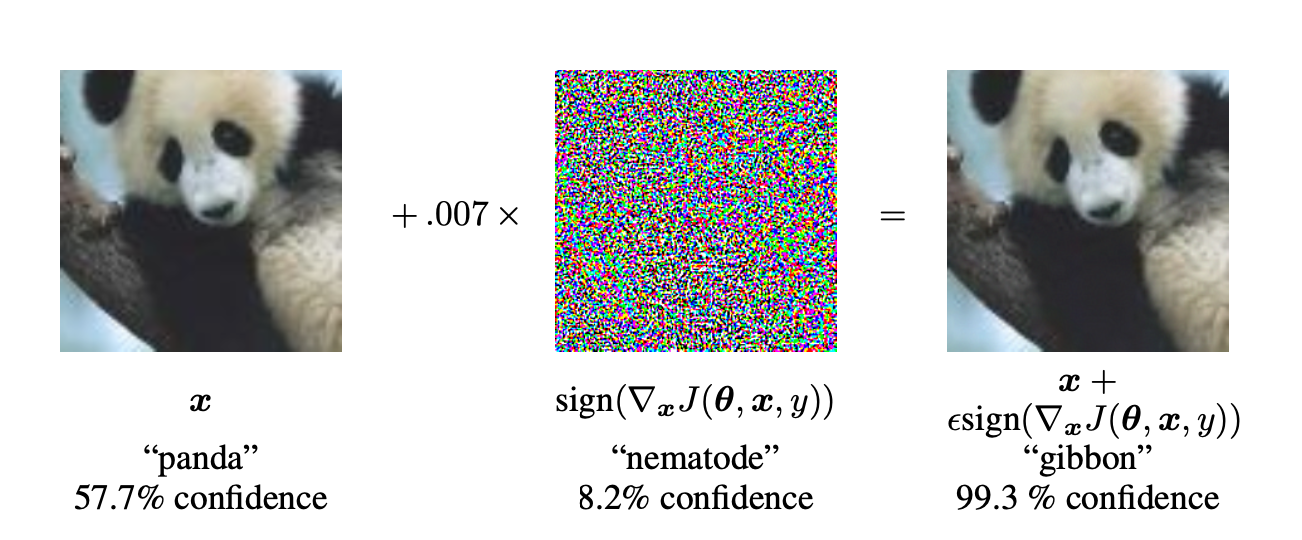
\includegraphics[width=13cm]{Definitions/fgsm.png}
\caption{Process of generating adversarial examples with FGSM.\label{fgsm}}
\end{figure} 

As shown in Figure~\ref{fgsm}, adversarial examples are generated using the gradient change that occurred during the training process.
At this time, \begin{math}\epsilon\end{math} is used to determine the degree of adversarial attack by reflecting the slope value.
In this paper, 0.05 and 0.1 were used as \begin{math}\epsilon\end{math}s. The failure to use values above 0.1 is due to the observation of human-obeservalbe transformation points in adversarial examples.
Therefore, if a value greater than 0.1, it can no longer serve as a adversarial example, so two types of \begin{math}\epsilon\end{math}s are used to generate adversarial examples.
In [], adversarial examples were applied only to the evaluation datas to confirm the effect of adversarial examples, but in our paper, training datas were also to create adversarial examples because adversarial examples should be used for training.

\begin{figure}[H]

\includegraphics[width=5 cm]{Definitions/logo-mdpi}
\caption{Examples of adversarial examples.\\(a) CIFAR-10 (b) CIFAR-100 (c)GTSRB\label{fig5}}
\end{figure} 

Through this method, as shown in Figure~\ref{fig5}, adversarial examples were generated for all data of CIFAR-10, CIFAR-100, and GTSRB to be used in the experiments.
In this paper, the training datas and evaluation datas which the adversarial attack is applied will be referred to as {\it adversarial training datas} and {\it adversarial evaluation datas}.
The generated adversarial training datas are randomly extracted at a certain ratio and mixed with the original training datas to be used for training. And the adversarial evalutaion datas are used for experiments to measure the safety.

\subsection{Methodology}

% 여기 보충 필요, 실험 방법에 대한 얘기는 하나도 안되있음
% 각각 실험에 대한 소개와 방법들에 대한 내용이 들어가야 한다.
We did experiments on the PC with Ubuntu 18.04 OS that had consisted of 4.20GHz Intel(R) i7-7700K CPU, 64GB RAM, and NVIDIA Titan XP 12GB GPU. The models used in the experiment have hyper parameters set to a batch size of 64, learning rate of 0.001, momentum of 0.9, CrossEntropy as loss functions and SGD as optimization functions, respectively.
Before proceeding with the training, we go through the process of mixing original train datas and the adversarial train datas generated from the result of section 4.2.
In this step, we trained the model only with the original train datas for being baseline of accuracy and safety performance, first. We then generate the mixed traniing dataset that mixes original train datas with adversarial train datas.
At this time, the mixing ratio was 8:2, 7:3, and 6:4 in total. When generating mixed dataset, the dataset was mixed by randomly extracting from each training datas according to the set ratio regardless of class.
The total number of datas in the mixed train datas is equal to the number of original train datas.

Once the training datas are ready, the model is trained. At this time, the hyper parameters of each model follow the aforementioned settings, and the training proceeds to the point where the accuracy becomes 90\% in the training process, storing the model at that time.

%%%%%%%%%%%%%%%%%%%%%%%%%%%%%%%%%%%%%%%%%%
\section{Experimental Results and Discussions}

In this paper, we hypothesized that adversarial training could significantly improve safety while minimizing the impact on performance, And we designed the experiments to prove this assumptions.
Chaper 5 summarized the results of the designed experiments and what can be learned through the experimental results.
Before discussing the experimental results, we defines some words in this chapter.
First, for datasets with any adversarial examples, it is called {\it orig}. Training datas and evaluation datas in {\it orig} were called {\it orig\_train} and {\it orig\_eval}.
For datasets with adversarial examples, it is called {\it adv}. Training datas and evaluation datas in {\it adv} were called {\it adv\_train} and {\it adv\_eval}.
These refer to each dataset and at the same time refer to the number of all datas contained in each dataset.
The {\it N model} means a model trainied on mixed training datas containing N\% of total number of traninig datas number of adversarial examples.
For example, a model trained with any adversarial training datas is called 0 model, and a model trained with mixed train datas which contains 20\% of the number of adversarial training datas is called 20 model.
{\it N model} evaluate each evaluation data. At this time the number of all correctly classified data is expressed by adding {\it correct} in front of each evaluation data.
For exmample, if evaluation data is {\it orig\_eval}, the number of all correctly classified data will be called {\it correct\_orig\_eval}.
At the same time, if evaluation data is {\it adv\_eval}, the number of all correctly classified data will be called {\it correct\_adv\_eval}.

We use accuracy and safety for experimental results measurement. Accuracy is a measure of how well the trained model classifies the {\it orig\_eval}, and can be defined as equation:

\begin{equation}
    acc(\%) = \text{{\it correct\_orig\_eval}} / \text{{\it orig\_eval}} \times 100
\end{equation} 

Safety is a measure of how well the trained model classifies the {\it adv\_eval}, and it can be defined as equation:

\begin{equation}
    safety(\%) = \text{{\it correct\_adv\_eval}} / \text{{\it adv\_eval}} \times 100
\end{equation}

Althogh the same equation is applied, we distinguish between the two measurements depending on whether the evaluation datas are in the {\it orig\_eval} or {\it adv\_eval}.

\subsection{CIFAR-10 Results}

\begin{specialtable}[H]
    \centering
    \caption{Results of CIFAR-10 with \begin{math}\epsilon\end{math}}
    \label{cifar10-result}
    {\small
    \begin{tabular}{|c|c|c|c|c|c|c|c|}
    \hline
    \multirow{2}{*}{Mixed Ratio} & \multirow{2}{*}{Matrix} & \multicolumn{3}{c|}{\begin{math}\epsilon\end{math}0.05}          & \multicolumn{3}{c|}{\begin{math}\epsilon\end{math} 0.1}         \\ \cline{3-8} 
                                 &                           & LeNet               & ResNet18              & VGG16              & LeNet              & ResNet18              & VGG16              \\ \hline
    \multirow{2}{*}{10:0}        & Acc                       & 63                  & 53                    & 78                 & 63                 & 53                    & 78                 \\ \cline{2-8} 
                                 & Safety                    & 18                  & 33                    & 33                 & 11                 & 27                    & 27                 \\ \hline
    \multirow{2}{*}{8:2}         & Acc                       & 60                  & 51                    & 73                 & 60                 & 50                    & 74                 \\ \cline{2-8} 
                                 & Safety                    & 45                  & 35                    & 56                 & 38                 & 31                    & 53                 \\ \hline
    \multirow{2}{*}{7:3}         & Acc                       & 58                  & 49                    & 72                 & 57                 & 49                    & 69                 \\ \cline{2-8} 
                                 & Safety                    & 45                  & 36                    & 56                 & 41                 & 34                    & 54                 \\ \hline
    \multirow{2}{*}{6:4}         & Acc                       & 58                  & 48                    & 70                 & 58                 & 47                    & 70                 \\ \cline{2-8} 
                                 & Safety                    & 47                  & 36                    & 56                 & 45                 & 34                    & 56                 \\ \hline
    \end{tabular}
    }
\end{specialtable}

Table~\ref{cifar10-result} shows the CIFAR-10 according to \begin{math}\epsilon\end{math} results for each model.

The results for the adversarial examples produced by \begin{math}\epsilon\end{math} 0.05 shows that the performance magnitude of accuracy and safety is significant, with 45\%  in LeNet, 20\% in ResNet18, and 45\% in VGG16.
Looking at the results of 0 model and 20 model, the accuracy decreased by 3\%(LeNet), 2\%(ResNet18), and 5\%(VGG16) for each model, but in the case of safety, it was improved by 27\%(LeNet), 2\%(ResNet18), and 23\%(VGG16) for each model.
Although the difference between 30 model and 40 model, the accuracy has slightly decreased compared to the 0 model, and the safety has been significantly improved.
Comparing 20 model, 30 model, and 40 model respectively, lower accuracy and higher safety were confirmed in the model with a high proportion of adversarial examples, but the differences were not large.
In reuslts for the adversarial examples produced by \begin{math}\epsilon\end{math} 0.1, as in \begin{math}\epsilon\end{math} 0.05, the accuracy of 20, 30, 40 model was slightly reduced compared to 0 model but a significant improvement in safety was achieved.

\begin{figure}[H]
    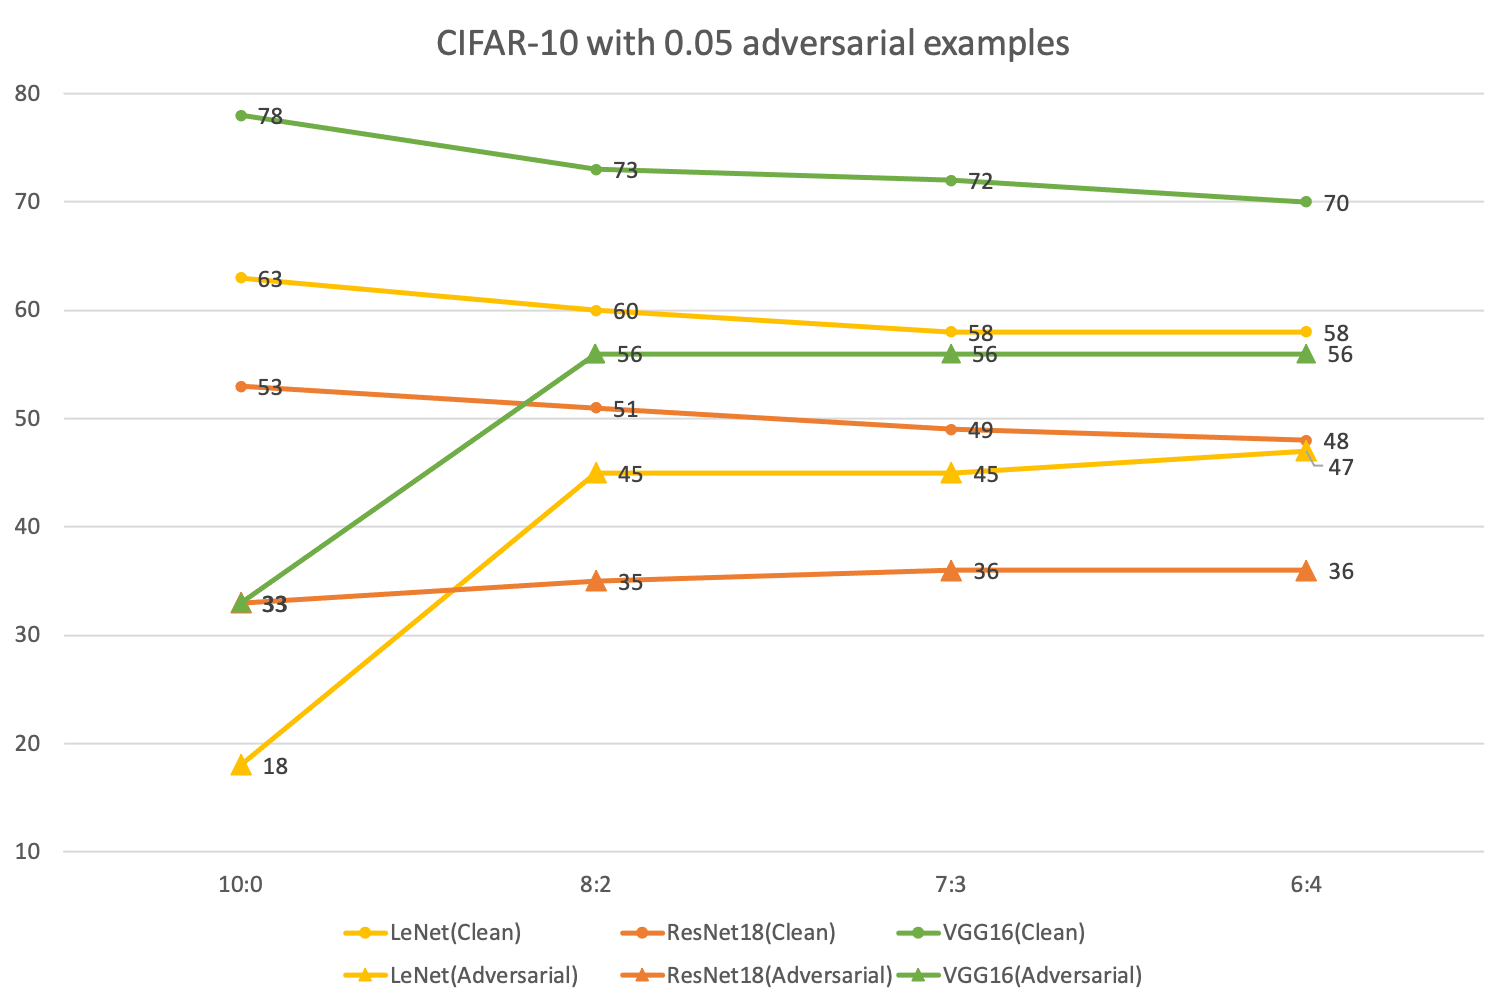
\includegraphics[width=13 cm]{Definitions/graph-005cifar10.png}
    \caption{Graphs of CIFAR-10 with \begin{math}\epsilon\end{math} 0.05\label{cifar10-0.05-graph}}
\end{figure}

This result can be better seen through Figure~\ref{cifar10-0.05-graph} and Figure~\ref{cifar10-0.1-graph} which graphically illustrated the table.
In Figure~\ref{cifar10-0.05-graph}, the results for the {\it adv\_eval} made with \begin{math}\epsilon\end{math} 0.05 can be visually confirmed.
As can be seen in the table, when adversarial examples are included at a higher rate, the accuracy is slightly decreased, but the safety is greatly improved.

\begin{figure}[H]
    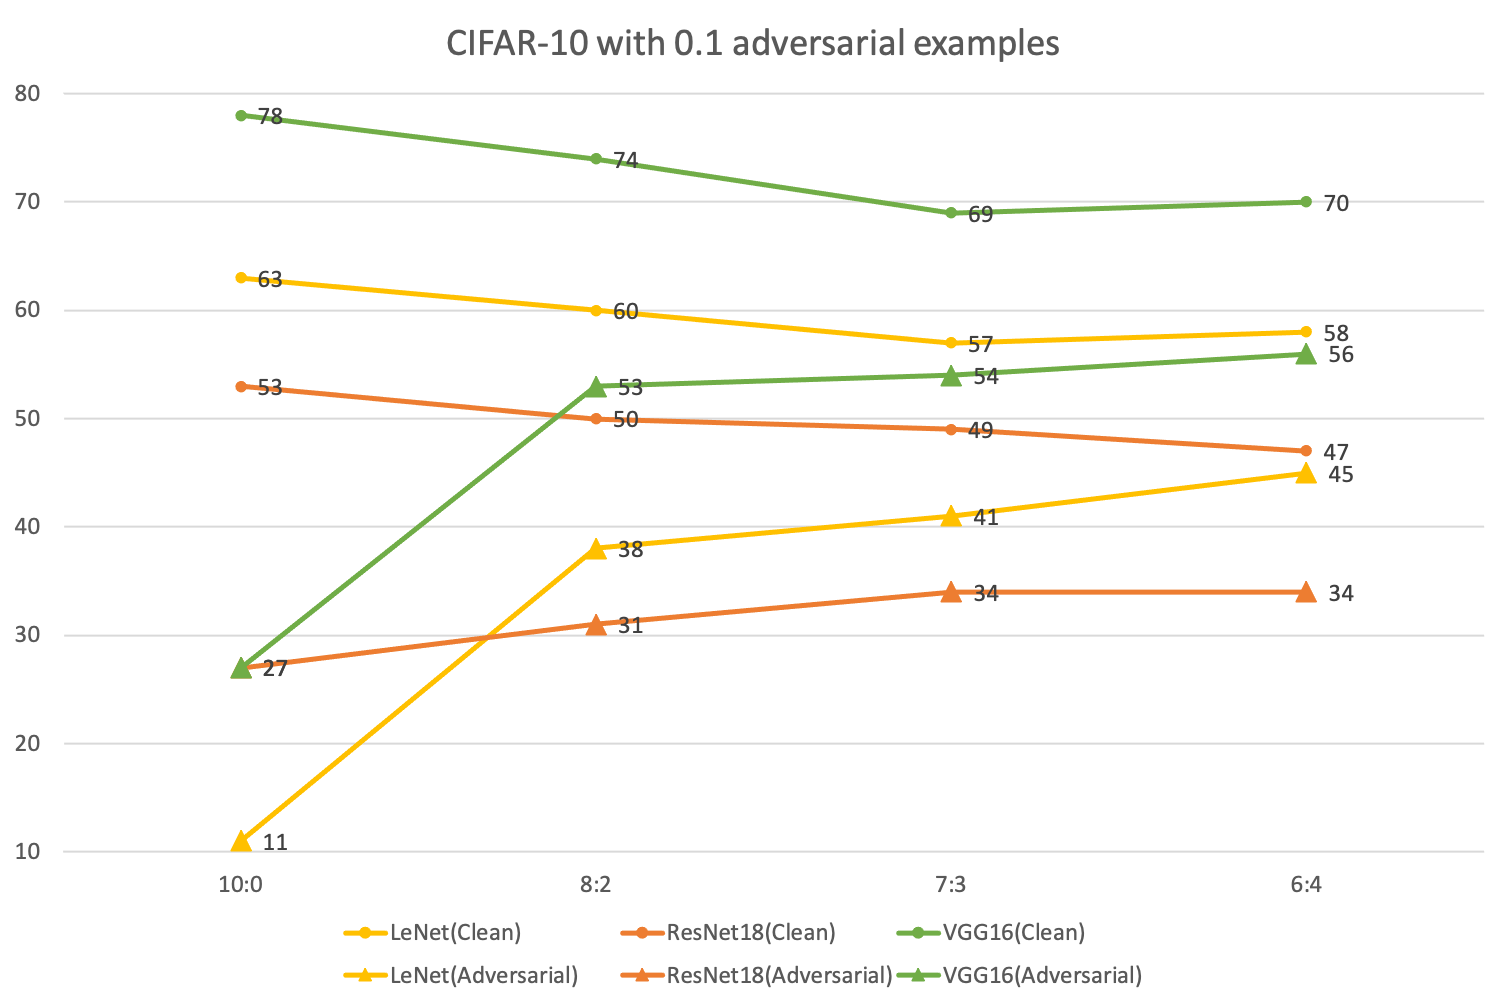
\includegraphics[width=13 cm]{Definitions/graph-01cifar10.png}
    \caption{Graphs of CIFAR-10 with \begin{math}\epsilon\end{math} 0.1\label{cifar10-0.1-graph}}
\end{figure}

In Figure~\ref{cifar10-0.1-graph}, the results for the {\it adv\_eval} made with \begin{math}\epsilon\end{math} 0.1 can be visually confirmed.
In Figure~\ref{cifar10-0.1-graph}, as in Figure~\ref{cifar10-0.05-graph}, changes in accuracy and safety can be seen as the ratio of containing adversarial examples increases.
% 아래부터 작업 시작
\subsection{CIFAR-100 Results}

\begin{specialtable}[H]
    \centering
    \caption{Results of CIFAR-100 with \begin{math}\epsilon\end{math}}
    \label{cifar100-results}
    {\small
    \begin{tabular}{|c|c|c|c|c|c|c|c|c|}
    \hline
    \multirow{2}{*}{Mixed Ratio} & \multirow{2}{*}{Matrix} & \multicolumn{3}{c|}{\begin{math}\epsilon \ 0.05\end{math}}& \multicolumn{3}{c|}{\begin{math}\epsilon \ 0.1\end{math}}       \\ \cline{3-8}
                                 &                           & LeNet               & ResNet18              & VGG16       & LeNet              & ResNet18              & VGG16              \\ \hline 
    \multirow{2}{*}{10:0}        & Acc                       & 63                  & 53                    & 78          & 63                 & 53                    & 78                 \\ \cline{2-8} 
                                 & Safety                    & 18                  & 33                    & 33          & 11                 & 27                    & 27                 \\ \hline 
    \multirow{2}{*}{8:2}         & Acc                       & 60                  & 51                    & 73          & 60                 & 50                    & 74                 \\ \cline{2-8} 
                                 & Safety                    & 45                  & 35                    & 56          & 38                 & 31                    & 53                 \\ \hline 
    \multirow{2}{*}{7:3}         & Acc                       & 58                  & 49                    & 72          & 57                 & 49                    & 69                 \\ \cline{2-8} 
                                 & Safety                    & 45                  & 36                    & 56          & 41                 & 34                    & 54                 \\ \hline 
    \multirow{2}{*}{6:4}         & Acc                       & 58                  & 48                    & 70          & 58                 & 47                    & 70                 \\ \cline{2-8} 
                                 & Safety                    & 47                  & 36                    & 56          & 45                 & 34                    & 56                 \\ \hline 
    \end{tabular}
    }
\end{specialtable}

Table~\ref{cifar100-results} shows the CIFAR-100 according to \begin{math}\epsilon\end{math} and the results for each model.

A first look at 0 model for the 0.05 \begin{math}\epsilon\end{math} adversarial examples shows a significant drop in accuracy comapred to CIFAR-10.
In the meantime, safety is much lower than accuracy. In particular, it can be seen that there is a difference of about 30\% in VGG16.
The reason that the accuracy is lower than that of CIFAR-10 is different characteristic of each dataset. The number of data for that class is small compared to the CIFAR-10, although the class has increased, so the degree of learning training under the same model conditions is different.
As with the experimental results of CIFAR-10, there is only a difference in the numericla value, and it can be confirmed that the accuracy is slightly decreased when the model is changed from 0 model to 20 model, but the safety performance is improved. 

\begin{figure}[H]
    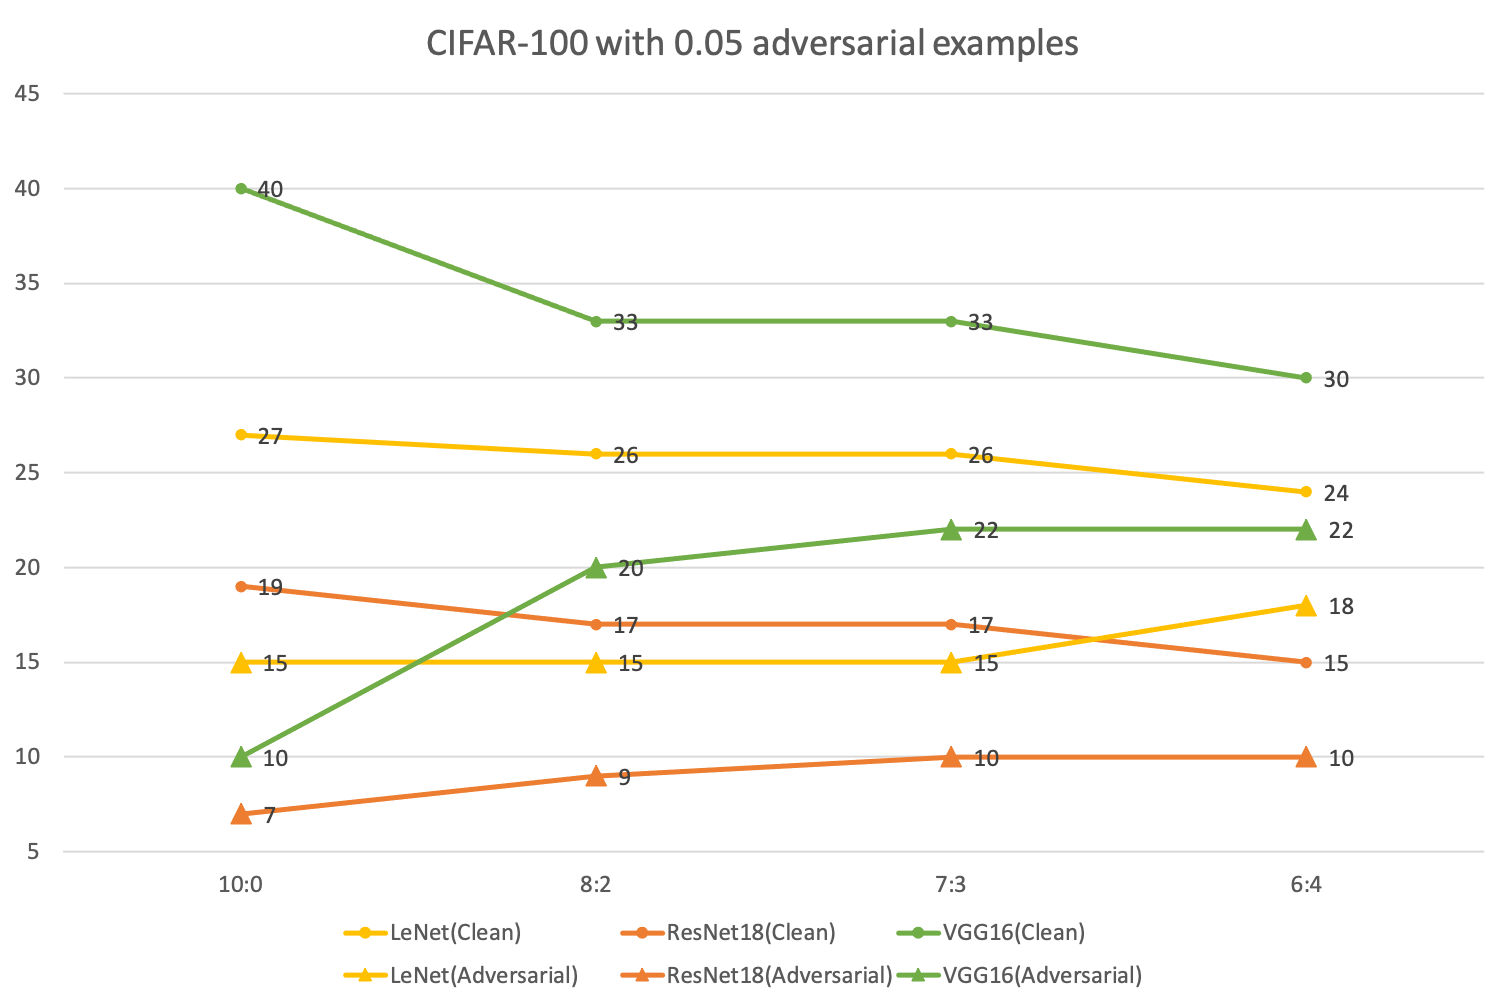
\includegraphics[width=13 cm]{Definitions/graph-005cifar100.png}
    \caption{Graphs of CIFAR-100 with \begin{math}\epsilon\end{math} 0.05\label{cifar100-0.05-graph}}
\end{figure} 

\begin{figure}[H]
    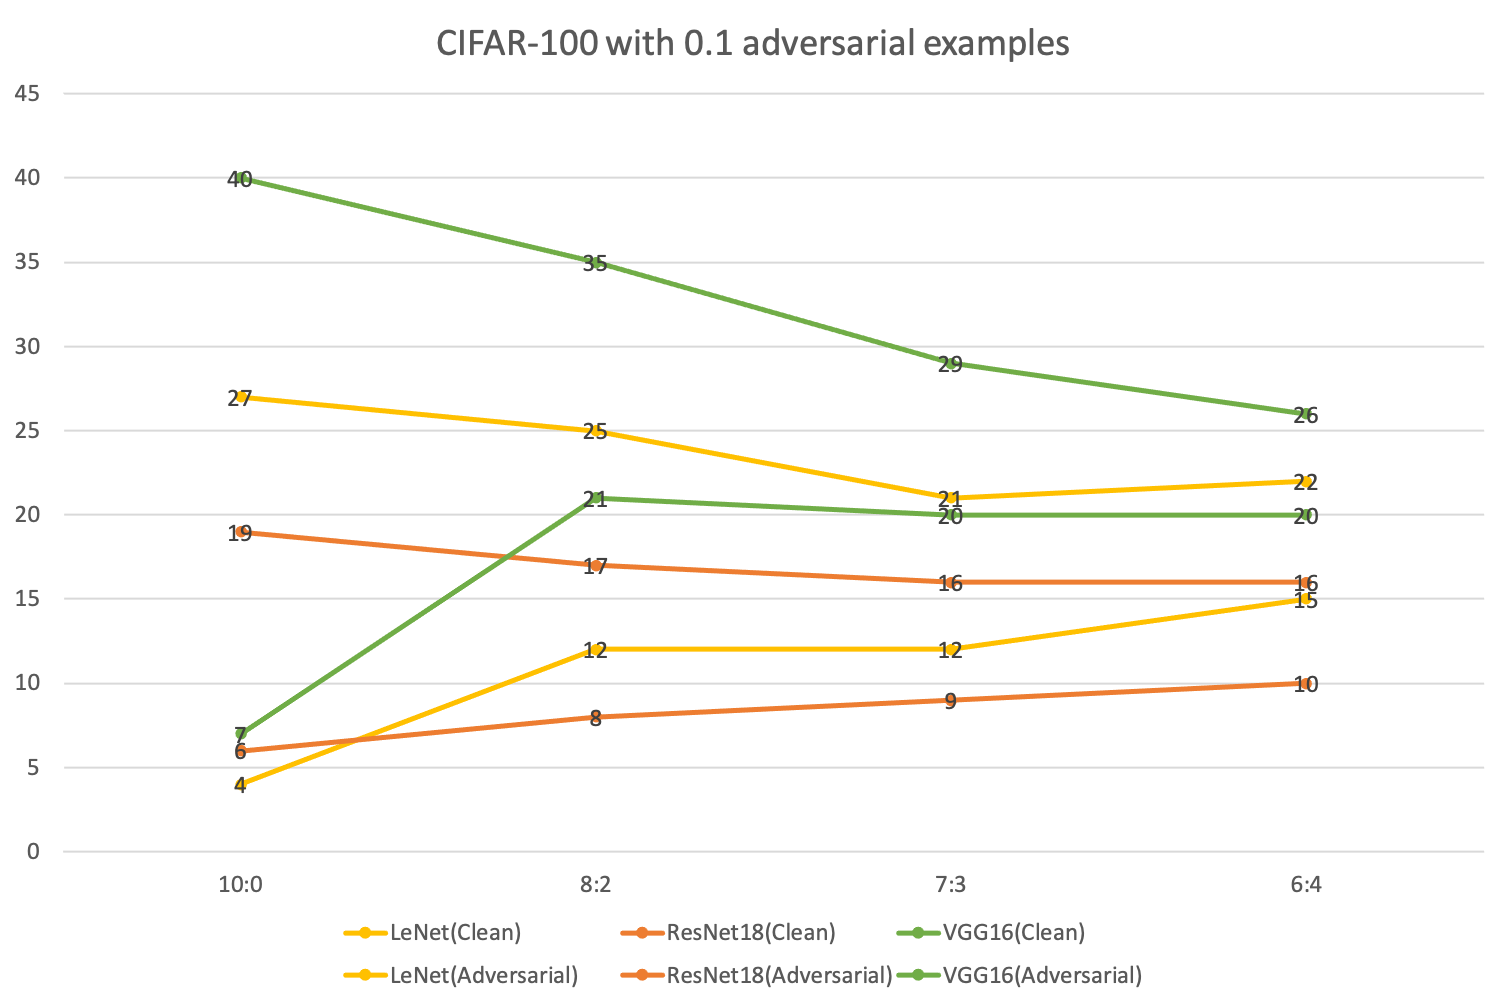
\includegraphics[width=13 cm]{Definitions/graph-01cifar100.png}
    \caption{Graphs of CIFAR-100 with \begin{math}\epsilon\end{math} 0.1\label{cifar100-0.1-graph}}
\end{figure} 

This can be seen visually through the figure~\ref{cifar10-0.05-graph} and figure~\ref{cifar10-0.1-graph}.

\subsection{GTSRB Results}

\begin{specialtable}[H]
    \centering
    \caption{Results of GTSRB with \begin{math}\epsilon\end{math}}
    \label{gtsrb-results}
    {\small
    \begin{tabular}{|c|c|c|c|c|c|c|c|c|}
    \hline
    \multirow{2}{*}{Mixed Ratio} & \multirow{2}{*}{Matrix} & \multicolumn{3}{c|}{\begin{math}\epsilon \ 0.05\end{math}}& \multicolumn{3}{c|}{\begin{math}\epsilon \ 0.1\end{math}}       \\ \cline{3-8}
                                 &                           & LeNet               & ResNet18              & VGG16       & LeNet              & ResNet18              & VGG16              \\ \hline 
    \multirow{2}{*}{10:0}        & Acc                       & 63                  & 53                    & 78          & 63                 & 53                    & 78                 \\ \cline{2-8} 
                                 & Safety                    & 18                  & 33                    & 33          & 11                 & 27                    & 27                 \\ \hline 
    \multirow{2}{*}{8:2}         & Acc                       & 60                  & 51                    & 73          & 60                 & 50                    & 74                 \\ \cline{2-8} 
                                 & Safety                    & 45                  & 35                    & 56          & 38                 & 31                    & 53                 \\ \hline 
    \multirow{2}{*}{7:3}         & Acc                       & 58                  & 49                    & 72          & 57                 & 49                    & 69                 \\ \cline{2-8} 
                                 & Safety                    & 45                  & 36                    & 56          & 41                 & 34                    & 54                 \\ \hline 
    \multirow{2}{*}{6:4}         & Acc                       & 58                  & 48                    & 70          & 58                 & 47                    & 70                 \\ \cline{2-8} 
                                 & Safety                    & 47                  & 36                    & 56          & 45                 & 34                    & 56                 \\ \hline 
    \end{tabular}
    }
\end{specialtable}

Table~\ref{gtsrb-results} shows the GTSRB according to \begin{math}\epsilon\end{math} and the results for each model.

Looking at the 0 model of thhe result for the 0.05 \begin{math}\epsilon\end{math} adversarial example first, it can be seen that the accuracy and safety performance are significantly different at 68\%(LeNet), 38\%(ResNet18), and 53\%(VGG16).
Similar to CIFAR datasets, we can see a very significnat improvement in safety performance from 0 model to 20 model.

\begin{figure}[H]
    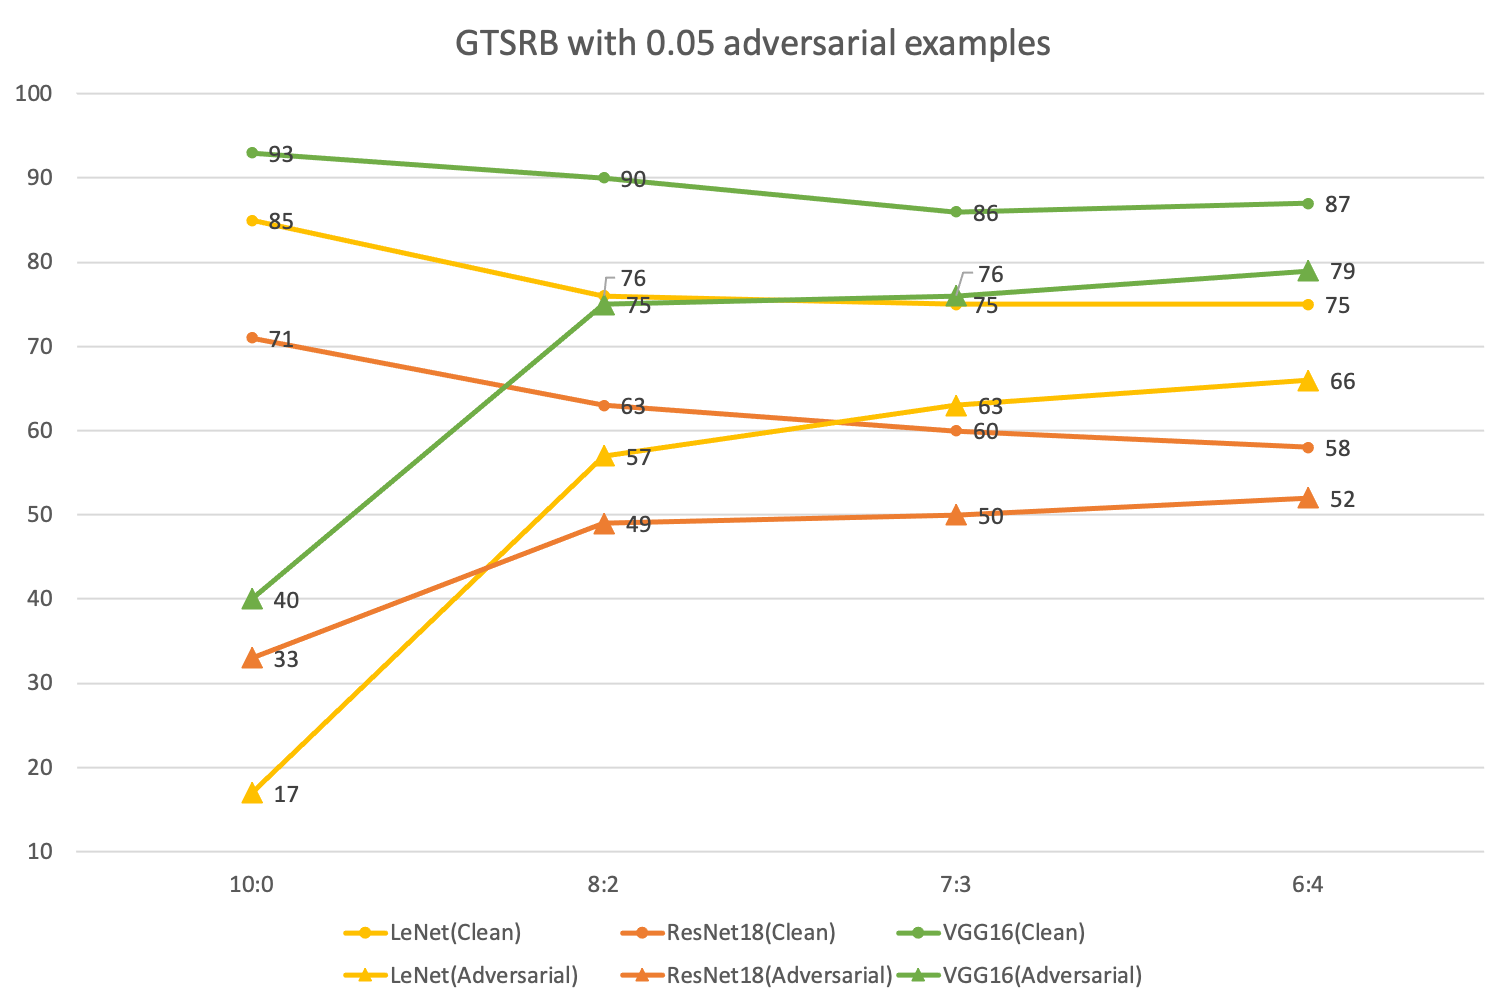
\includegraphics[width=13 cm]{Definitions/graph-005gtsrb.png}
    \caption{Graphs of GTSRB with \begin{math}\epsilon\end{math} 0.05\label{gtsrb-0.05-graph}}
\end{figure} 

\begin{figure}[H]
    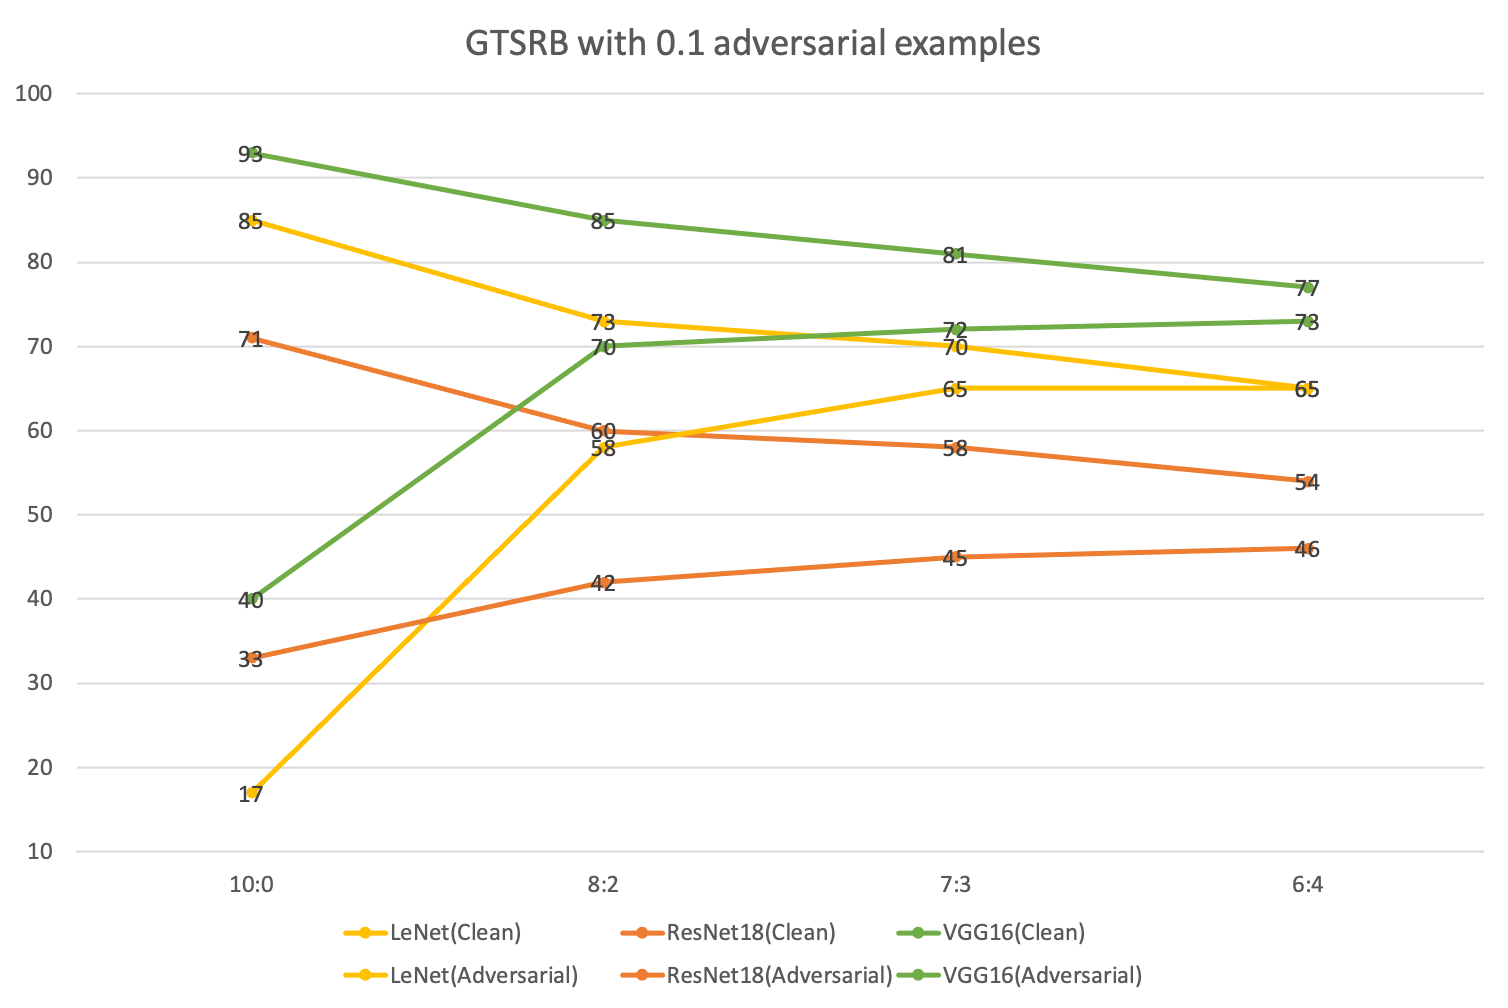
\includegraphics[width=13 cm]{Definitions/graph-01gtsrb.png}
    \caption{Graphs of GTSRB with \begin{math}\epsilon\end{math} 0.1\label{gtsrb-0.1-graph}}
\end{figure} 

It can be visually confirmed through figure~\ref{gtsrb-0.05-graph} and figure~\ref{gtsrb-0.1-graph}.
In figure~\ref{gtsrb-0.05-graph} and figure~\ref{gtsrb-0.1-graph} as with the CIFAR datasets, the improvement in safety is much larger than the decrease in accuracy, and it can be seen that there is a slight difference between models with adversarial examples.

\subsection{Discussion} % 네트워크 구조 영향에 대한 해석 추가

% 실험 결과가 이러이러 했으므로 우리는 이런 프로세스를 제안할 것이다.
% 기존 소프트웨어의 경우 데이터 준비를 하고 학습 및 평가를 진행하고 이후 피드백 과정을 통해서 모델을 정제하였다.
% 우리 모델에서는 데이터 준비 단계에서 적대적 예시 포함 비율 여부와 같은 것을 검증함을 통해서 1차적으로 검증을 들어가고 학습하기 때문에 필요한 피드백을 최소 1회 줄일 수 있다.
% 이를 통해 다음과 같은 프로세스를 제안한다.

The interpretation of the experimental results according to 3 different datasets and models and various experimental conditions and the answer to the RQs in the thesis can be confirmed as follows. \\

For all datasets, it can be seen that the safety of 0 model has a large performance difference compared to the accuracy. This confirms that the generated adversarial examples were properly generated. \\

RQ1 was the question of whether adversarial training well classifies adversarial examples of classification models.
In experiemnts using the CIFAR datasets, it was confirmed that the safety performance of 20 model, 30 model and 40 model including the adversarial examples was significantly improved compared to the safety of 0 model not including the adversarial examples.
Through this, it was confirmed that adversarial training can contribute to the improvement of the safety performance of the classification model.
However, in the CIFAR-100, training was not sufficient during epoch, resulting in lower values, but the performance change tendency itself observed in 0 model and the rest of the models could be ovserved in the same way.

RQ2 is an extended question from RQ1, as to whether the dataset used in the experiemnt could have the same effect even if it was a dataset related to safety.
In the experiemntal results using the GTSRB, similar to the results of the CIFAR datasets, it was confirmed that the safety was significantly improved in the 20 model, 30 model and 40 model compared to 0 model.

RQ3 was a question of what ration would be the best performance to mix adversarial examples with original datas to form a mixed training dataset.
This depends on the dataset used and whether the requirements they value are accuracy or safety, but in this paper we mainly looked at the performance balance between accuracy and safety.
In the experiemnts, it can be seen that it is essential to mix the adversarial examples from training datas at least 20\% when contruct the training dataset in order to verify the safety.
This is because the greatest improvement in safety can be obtained compared to 0 model when 20 model is used in all experimental environments.
Even if adversarial training data is included at a higher rate than that, the degree of safety improvement is small, so it can be considered as the minimum requirements to configuer 20\% of the total training dataset as adversarial examples.
If accuracy is considered a more important requirements, the proportion of adversarial examples can be reduced, and if safety is considered a more important requirement, more adversarial examples can be included.

Additionally, in graphs, it can be seen that the shape of the graph shows the same tendency for all datasets and different \begin{math}\epsilon\end{math}.
Through this, it was confirmed that, regardless of the degree of deformation of the adversarial example, adversarial training can lead to improved safety.

% 이 그림에 대한 해석
% 그냥 데이터만으로 학습을 진행하고 데이터 셋을 정제하거나 모델을 파인튠한 기존 프로세스
% 데이터 준비 단계에서 적대적 예시 데이터 셋을 활용하여 결과에서 데이터 셋 정제하거나 모델 파인튠에 사용할 수 있는 부가적인 정보를 얻을 수 있는 우리의구조
\begin{figure}[H]
    
\includegraphics[width=13 cm]{Definitions/comparison.png}
    \caption{Comparison between existing process and our process\label{comparison}}
\end{figure} 

To summarize the experimental results, adversarial training can contribute to improving the safety of the classificatio model, which also applies to safety-reslated datasets.
In order to verify safety, it is recommended that at least 20\% of the training data consist of adversarial examples, and it can be proved that it can help to verify the desired requirements by adjusting the inclusion ratio of adversarial exampels according to priority among accuracy and safety.

%%%%%%%%%%%%%%%%%%%%%%%%%%%%%%%%%%%%%%%%%%
\section{Conclusions}

We have confirmed through experiments that adversarial training can improve the safety performance with little effect on accuracy of the model.
This means that generating adversarial examples using the dataset you have before proceeding with learning and including the adversarial examples in the training dataset can be used as one of the factors that can verify the safety of AI.
Furthermore, we proposed the method to achieve a balance between accuracy and safety for the dataset used in the experiments by generating a mixed dataset of different ratios.
It can be used as a methodology that can balance the performance between accuracy and safety by performing the experimental method proposed in the thesis several times according to the important requirements and adjusting the ratio of inclusion of adversarial examples in training dataset.
Based on the proposed methods, when entering into an actual AI project, it can be used as one of the factors that can verify the safety before the training process that consumes a lot of resources by checking whether adversarial examples are included in the training dataset. Therefore, it is possible to reduce the resources required for at least one tarninig.
Moreover, it is possible to reduce the cost of training model that verifies the requirements by adjusting the ratio of inclusion of adversarial examples for higher-value requirements through accuracy and safety after one training and evaluation.

In future work, we plan to verify the validity of the proposed method for more diverse classification datasets, different model structures, and various adversarial attack methods.
In addition, we are going to conduct research on how NFRs other than AI and safety for purposes other than classification models can be pre-verified through experiements.

%%%%%%%%%%%%%%%%%%%%%%%%%%%%%%%%%%%%%%%%%%
\section{Patents}

This section is not mandatory, but may be added if there are patents resulting from the work reported in this manuscript.

%%%%%%%%%%%%%%%%%%%%%%%%%%%%%%%%%%%%%%%%%%
\vspace{6pt} 

%%%%%%%%%%%%%%%%%%%%%%%%%%%%%%%%%%%%%%%%%%
%% optional
%\supplementary{The following are available online at \linksupplementary{s1}, Figure S1: title, Table S1: title, Video S1: title.}

% Only for the journal Methods and Protocols:
% If you wish to submit a video article, please do so with any other supplementary material.
% \supplementary{The following are available at \linksupplementary{s1}, Figure S1: title, Table S1: title, Video S1: title. A supporting video article is available at doi: link.} 

%%%%%%%%%%%%%%%%%%%%%%%%%%%%%%%%%%%%%%%%%%
\authorcontributions{For research articles with several authors, a short paragraph specifying their individual contributions must be provided. The following statements should be used ``Conceptualization, X.X. and Y.Y.; methodology, X.X.; software, X.X.; validation, X.X., Y.Y. and Z.Z.; formal analysis, X.X.; investigation, X.X.; resources, X.X.; data curation, X.X.; writing---original draft preparation, X.X.; writing---review and editing, X.X.; visualization, X.X.; supervision, X.X.; project administration, X.X.; funding acquisition, Y.Y. All authors have read and agreed to the published version of the manuscript.'', please turn to the  \href{http://img.mdpi.org/data/contributor-role-instruction.pdf}{CRediT taxonomy} for the term explanation. Authorship must be limited to those who have contributed substantially to the work~reported.}

\funding{Please add: ``This research received no external funding'' or ``This research was funded by NAME OF FUNDER grant number XXX.'' and  and ``The APC was funded by XXX''. Check carefully that the details given are accurate and use the standard spelling of funding agency names at \url{https://search.crossref.org/funding}, any errors may affect your future funding.}

\institutionalreview{In this section, please add the Institutional Review Board Statement and approval number for studies involving humans or animals. Please note that the Editorial Office might ask you for further information. Please add ``The study was conducted according to the guidelines of the Declaration of Helsinki, and approved by the Institutional Review Board (or Ethics Committee) of NAME OF INSTITUTE (protocol code XXX and date of approval).'' OR ``Ethical review and approval were waived for this study, due to REASON (please provide a detailed justification).'' OR ``Not applicable'' for studies not involving humans or animals. You might also choose to exclude this statement if the study did not involve humans or animals.}

\informedconsent{Any research article describing a study involving humans should contain this statement. Please add ``Informed consent was obtained from all subjects involved in the study.'' OR ``Patient consent was waived due to REASON (please provide a detailed justification).'' OR ``Not applicable'' for studies not involving humans. You might also choose to exclude this statement if the study did not involve humans.

Written informed consent for publication must be obtained from participating patients who can be identified (including by the patients themselves). Please state ``Written informed consent has been obtained from the patient(s) to publish this paper'' if applicable.}

\dataavailability{In this section, please provide details regarding where data supporting reported results can be found, including links to publicly archived datasets analyzed or generated during the study. Please refer to suggested Data Availability Statements in section ``MDPI Research Data Policies'' at \url{https://www.mdpi.com/ethics}. You might choose to exclude this statement if the study did not report any data.} 

\acknowledgments{In this section you can acknowledge any support given which is not covered by the author contribution or funding sections. This may include administrative and technical support, or donations in kind (e.g., materials used for experiments).}

\conflictsofinterest{Declare conflicts of interest or state ``The authors declare no conflict of interest.'' Authors must identify and declare any personal circumstances or interest that may be perceived as inappropriately influencing the representation or interpretation of reported research results. Any role of the funders in the design of the study; in the collection, analyses or interpretation of data; in the writing of the manuscript, or in the decision to publish the results must be declared in this section. If there is no role, please state ``The funders had no role in the design of the study; in the collection, analyses, or interpretation of data; in the writing of the manuscript, or in the decision to publish the~results''.} 

%% Optional
\sampleavailability{Samples of the compounds ... are available from the authors.}

%%%%%%%%%%%%%%%%%%%%%%%%%%%%%%%%%%%%%%%%%%
%% Only for journal Encyclopedia
%\entrylink{The Link to this entry published on the encyclopedia platform.}

%%%%%%%%%%%%%%%%%%%%%%%%%%%%%%%%%%%%%%%%%%
%% Optional
\abbreviations{Abbreviations}{
The following abbreviations are used in this manuscript:\\

\noindent 
\begin{tabular}{@{}ll}
MDPI & Multidisciplinary Digital Publishing Institute\\
DOAJ & Directory of open access journals\\
TLA & Three letter acronym\\
LD & Linear dichroism
\end{tabular}}

%%%%%%%%%%%%%%%%%%%%%%%%%%%%%%%%%%%%%%%%%%
%% Optional
\appendixtitles{no} % Leave argument "no" if all appendix headings stay EMPTY (then no dot is printed after "Appendix A"). If the appendix sections contain a heading then change the argument to "yes".
\appendixstart
\appendix
\section{}
\subsection{}
The appendix is an optional section that can contain details and data supplemental to the main text---for example, explanations of experimental details that would disrupt the flow of the main text but nonetheless remain crucial to understanding and reproducing the research shown; figures of replicates for experiments of which representative data are shown in the main text can be added here if brief, or as Supplementary Data. Mathematical proofs of results not central to the paper can be added as an appendix.

\section{}
All appendix sections must be cited in the main text. In the appendices, Figures, Tables, etc. should be labeled, starting with ``A''---e.g., Figure A1, Figure A2, etc. 

%%%%%%%%%%%%%%%%%%%%%%%%%%%%%%%%%%%%%%%%%%
\end{paracol}
%%%%%%%%%%%%%%%%%%%%%%%%%%%%%%%%%%%%%%%%%%
% To add notes in main text, please use \endnote{} and un-comment the codes below.
%\begin{adjustwidth}{-5.0cm}{0cm}
%\printendnotes[custom]
%\end{adjustwidth}
%%%%%%%%%%%%%%%%%%%%%%%%%%%%%%%%%%%%%%%%%%
\reftitle{References}

% Please provide either the correct journal abbreviation (e.g. according to the “List of Title Word Abbreviations” http://www.issn.org/services/online-services/access-to-the-ltwa/) or the full name of the journal.
% Citations and References in Supplementary files are permitted provided that they also appear in the reference list here. 

%=====================================
% References, variant A: external bibliography
%=====================================
%\externalbibliography{yes}
%\bibliography{your_external_BibTeX_file}

%=====================================
% References, variant B: internal bibliography
%=====================================
\begin{thebibliography}{999}
% Reference 1
\bibitem[Author1(year)]{ref-journal}
Author~1, T. The title of the cited article. {\em Journal Abbreviation} {\bf 2008}, {\em 10}, 142--149.
% Reference 2
\bibitem[Author2(year)]{ref-book1}
Author~2, L. The title of the cited contribution. In {\em The Book Title}; Editor1, F., Editor2, A., Eds.; Publishing House: City, Country, 2007; pp. 32--58.
% Reference 3
\bibitem[Author3(year)]{ref-book2}
Author 1, A.; Author 2, B. \textit{Book Title}, 3rd ed.; Publisher: Publisher Location, Country, 2008; pp. 154--196.
% Reference 4
\bibitem[Author4(year)]{ref-unpublish}
Author 1, A.B.; Author 2, C. Title of Unpublished Work. \textit{Abbreviated Journal Name} stage of publication (under review; accepted; in~press).
% Reference 5
\bibitem[Author5(year)]{ref-communication}
Author 1, A.B. (University, City, State, Country); Author 2, C. (Institute, City, State, Country). Personal communication, 2012.
% Reference 6
\bibitem[Author6(year)]{ref-proceeding}
Author 1, A.B.; Author 2, C.D.; Author 3, E.F. Title of Presentation. In Title of the Collected Work (if available), Proceedings of the Name of the Conference, Location of Conference, Country, Date of Conference; Editor 1, Editor 2, Eds. (if available); Publisher: City, Country, Year (if available); Abstract Number (optional), Pagination (optional).
% Reference 7
\bibitem[Author7(year)]{ref-thesis}
Author 1, A.B. Title of Thesis. Level of Thesis, Degree-Granting University, Location of University, Date of Completion.
% Reference 8
\bibitem[Author8(year)]{ref-url}
Title of Site. Available online: URL (accessed on Day Month Year).
\end{thebibliography}

% If authors have biography, please use the format below
%\section*{Short Biography of Authors}
%\bio
%{\raisebox{-0.35cm}{\includegraphics[width=3.5cm,height=5.3cm,clip,keepaspectratio]{Definitions/author1.pdf}}}
%{\textbf{Firstname Lastname} Biography of first author}
%
%\bio
%{\raisebox{-0.35cm}{\includegraphics[width=3.5cm,height=5.3cm,clip,keepaspectratio]{Definitions/author2.jpg}}}
%{\textbf{Firstname Lastname} Biography of second author}

% The following MDPI journals use author-date citation: Admsci,  Arts, Econometrics, Economies, Genealogy, Humanities, IJFS, Jintelligence, JRFM, Languages, Laws, Literature, Religions, Risks, Social Sciences. For those journals, please follow the formatting guidelines on http://www.mdpi.com/authors/references
% To cite two works by the same author: \citeauthor{ref-journal-1a} (\citeyear{ref-journal-1a}, \citeyear{ref-journal-1b}). This produces: Whittaker (1967, 1975)
% To cite two works by the same author with specific pages: \citeauthor{ref-journal-3a} (\citeyear{ref-journal-3a}, p. 328; \citeyear{ref-journal-3b}, p.475). This produces: Wong (1999, p. 328; 2000, p. 475)

%%%%%%%%%%%%%%%%%%%%%%%%%%%%%%%%%%%%%%%%%%
%% for journal Sci
%\reviewreports{\\
%Reviewer 1 comments and authors’ response\\
%Reviewer 2 comments and authors’ response\\
%Reviewer 3 comments and authors’ response
%}
%%%%%%%%%%%%%%%%%%%%%%%%%%%%%%%%%%%%%%%%%%
\end{document}

